\documentclass[]{article}
\usepackage{amsmath}
\usepackage{amsfonts} 
\usepackage[english]{babel}
\usepackage{amsthm}
\usepackage{bbm}  % for indicator functions and stuff. 
\usepackage{mathtools}
\usepackage{hyperref}
% \usepackage{minted}
% Basic Type Settings ----------------------------------------------------------
\usepackage[margin=1in,footskip=0.25in]{geometry}
\linespread{1}  % double spaced or single spaced
\usepackage[fontsize=12pt]{fontsize}

\theoremstyle{definition}
\newtheorem{theorem}{Theorem}       % Theorem counter global 
\newtheorem{prop}{Proposition}[section]  % proposition counter is section
\newtheorem{lemma}{Lemma}[subsection]  % lemma counter is subsection
\newtheorem{definition}{Definition}
\newtheorem{remark}{Remark}[subsection]


\hypersetup{
    colorlinks=true,
    linkcolor=blue,
    filecolor=magenta,
    urlcolor=cyan,
}
\usepackage[final]{graphicx}
\usepackage{listings}
\usepackage{courier}
\lstset{basicstyle=\footnotesize\ttfamily,breaklines=true}
\newcommand{\indep}{\perp \!\!\! \perp}
\usepackage{wrapfig}
\graphicspath{{.}}
\usepackage{fancyvrb}

%%
%% Julia definition (c) 2014 Jubobs
%%
\usepackage[T1]{fontenc}
\usepackage{beramono}
\usepackage[usenames,dvipsnames]{xcolor}
\lstdefinelanguage{Julia}%
  {morekeywords={abstract,break,case,catch,const,continue,do,else,elseif,%
      end,export,false,for,function,immutable,import,importall,if,in,%
      macro,module,otherwise,quote,return,switch,true,try,type,typealias,%
      using,while},%
   sensitive=true,%
   alsoother={$},%
   morecomment=[l]\#,%
   morecomment=[n]{\#=}{=\#},%
   morestring=[s]{"}{"},%
   morestring=[m]{'}{'},%
}[keywords,comments,strings]%
\lstset{%
    language         = Julia,
    basicstyle       = \ttfamily,
    keywordstyle     = \bfseries\color{blue},
    stringstyle      = \color{magenta},
    commentstyle     = \color{ForestGreen},
    showstringspaces = false,
}



\begin{document}
\numberwithin{equation}{subsection}
\section{Notations}
\begin{enumerate}
    \item $\delta^+(v)$ is the set of arcs that are coming out of $v$, $\delta^-(v)$ is the set of arcs that are coming into the vertex $v$. 
    \item $\mathbbm 1_M$ is the indicator vector of some sets. In the case of graph, let $M$ be a set of edges, then $\mathbbm 1_M \in \mathbb R^{|E|}$ and $(\mathbbm 1_{M})_e = 1$ if $e \in M$ else it's just zero. 
\end{enumerate}
\section{Problem 4.10}
    Determine using the max flow algorithm if thre exists a $3\times 3$ matrix whose row sum is $\le [13, 9, 4]$ and whose column sum is $= [3, 7, 12]$ and the matrix is: 
    \begin{align}
        A \le \begin{bmatrix}
            2 & 0 & 8 \\
            3 & 8 & 3 \\
            0 & 1 & 3
        \end{bmatrix}
    \end{align}
    \subsection{Reduction Strategies}
        There are 3 sets of inequalities, each corresponds to the capacity limit of each edges on the graph, in addition. The summation happens at the vertices. 
        \par
        Entries of the matrix can be modeled by edges going between 2 sets of bipartite graph. On each side of the bipartite graph we connect the $s, t$ vertices, and we link $s, t$ to each vertices in each group by one edge, and those edges corresponds to the row sum and the column sum. 
        \begin{figure}[h]
            \centering
            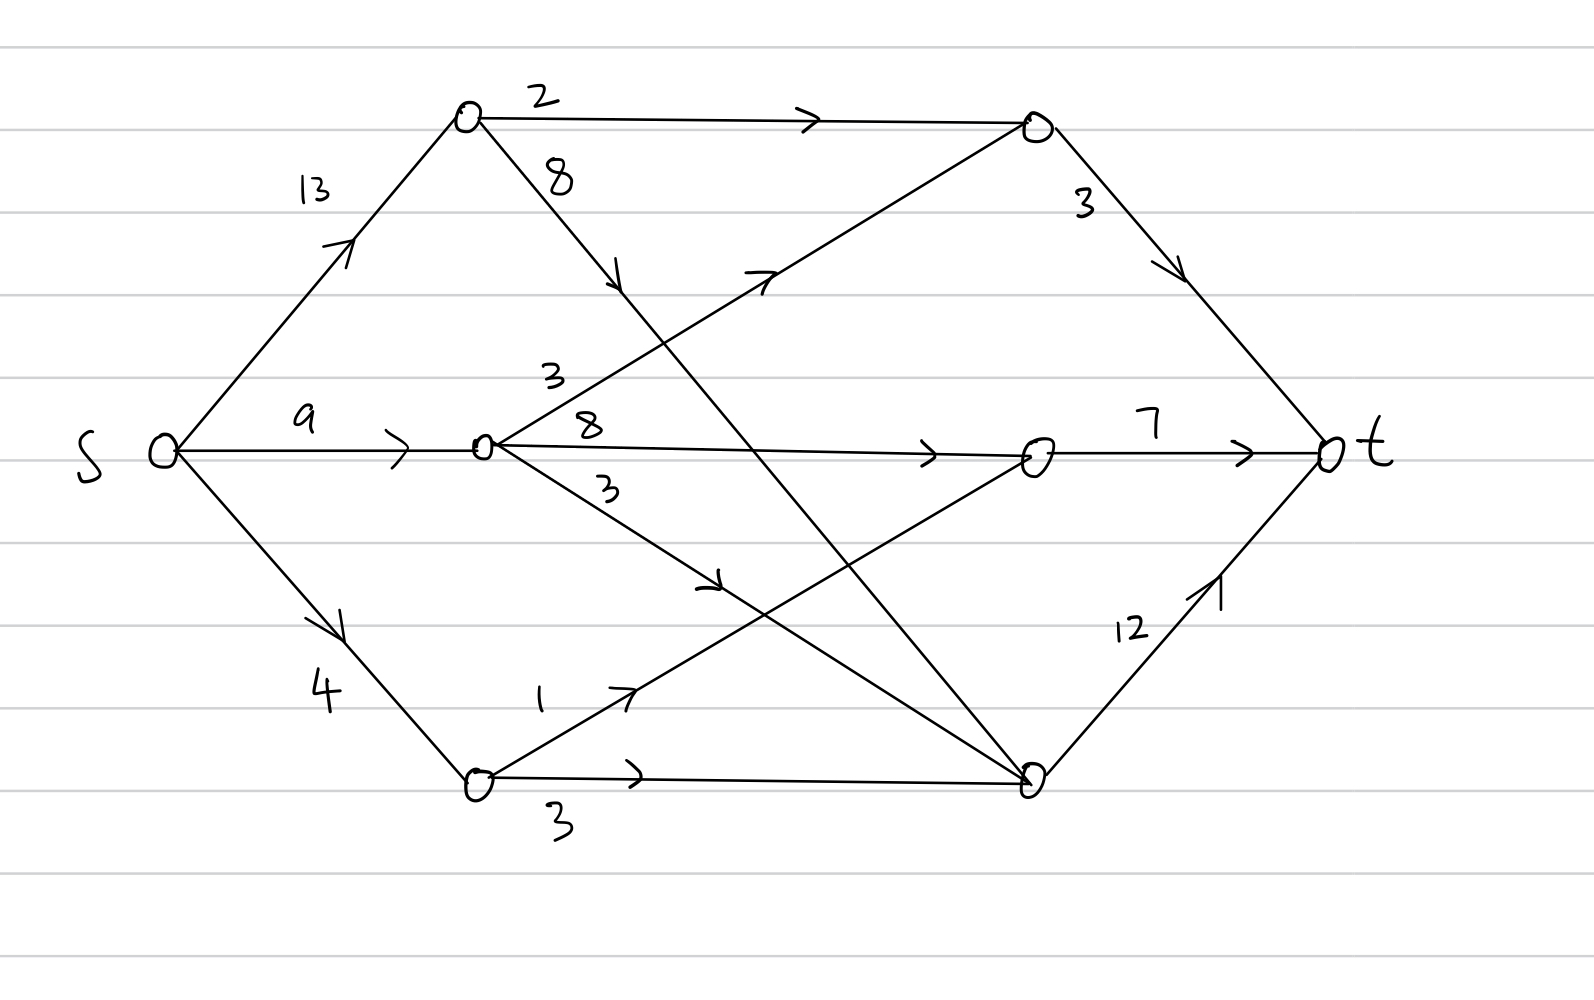
\includegraphics[width=14cm]{reduced_graph.jpeg}
        \end{figure}
        The matrix $A$ exists iff there is a way to send flow on the above graph such that the value of the flow equals to $3 + 7 + 12$, saturating all the edges coming into the vertex $t$. 
    \newpage
    \subsection{Applying Network Algorithm}
        Actually solving the flow by hands:
        \begin{figure}
            \centering
            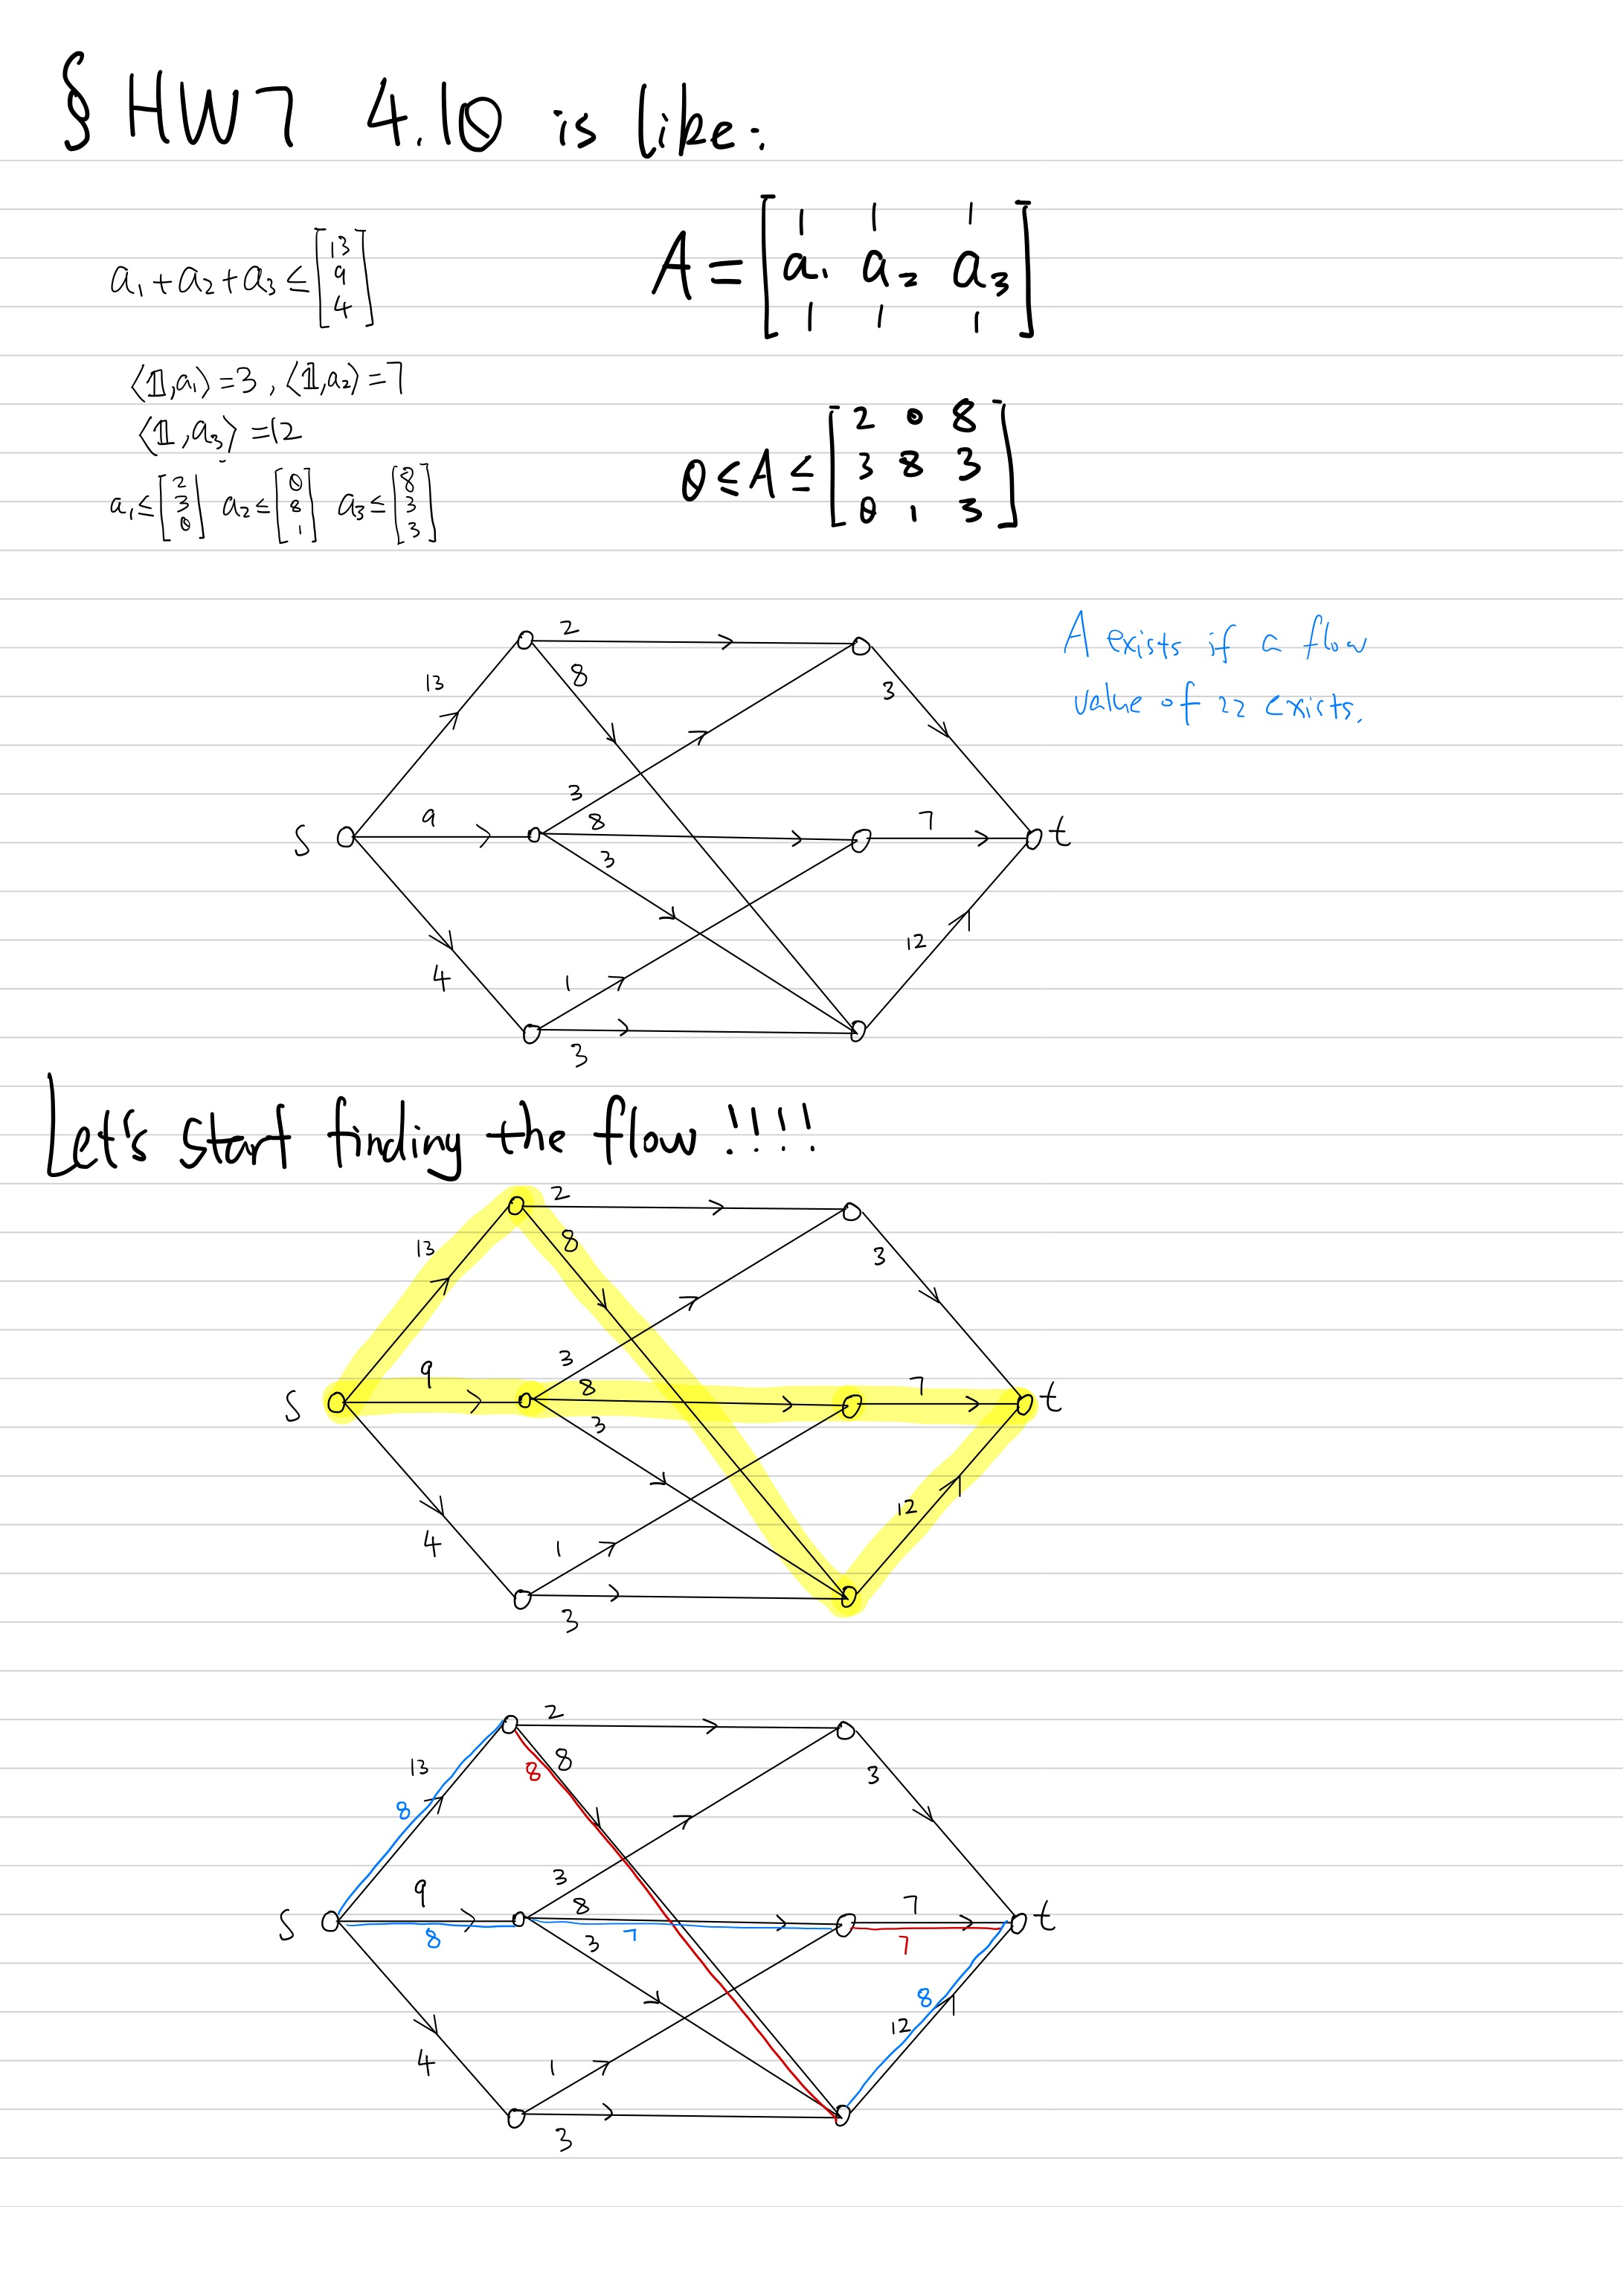
\includegraphics[width=14cm]{Settled Results Ready to Transfer-5.jpg}
        \end{figure}
        \begin{figure}
            \centering
            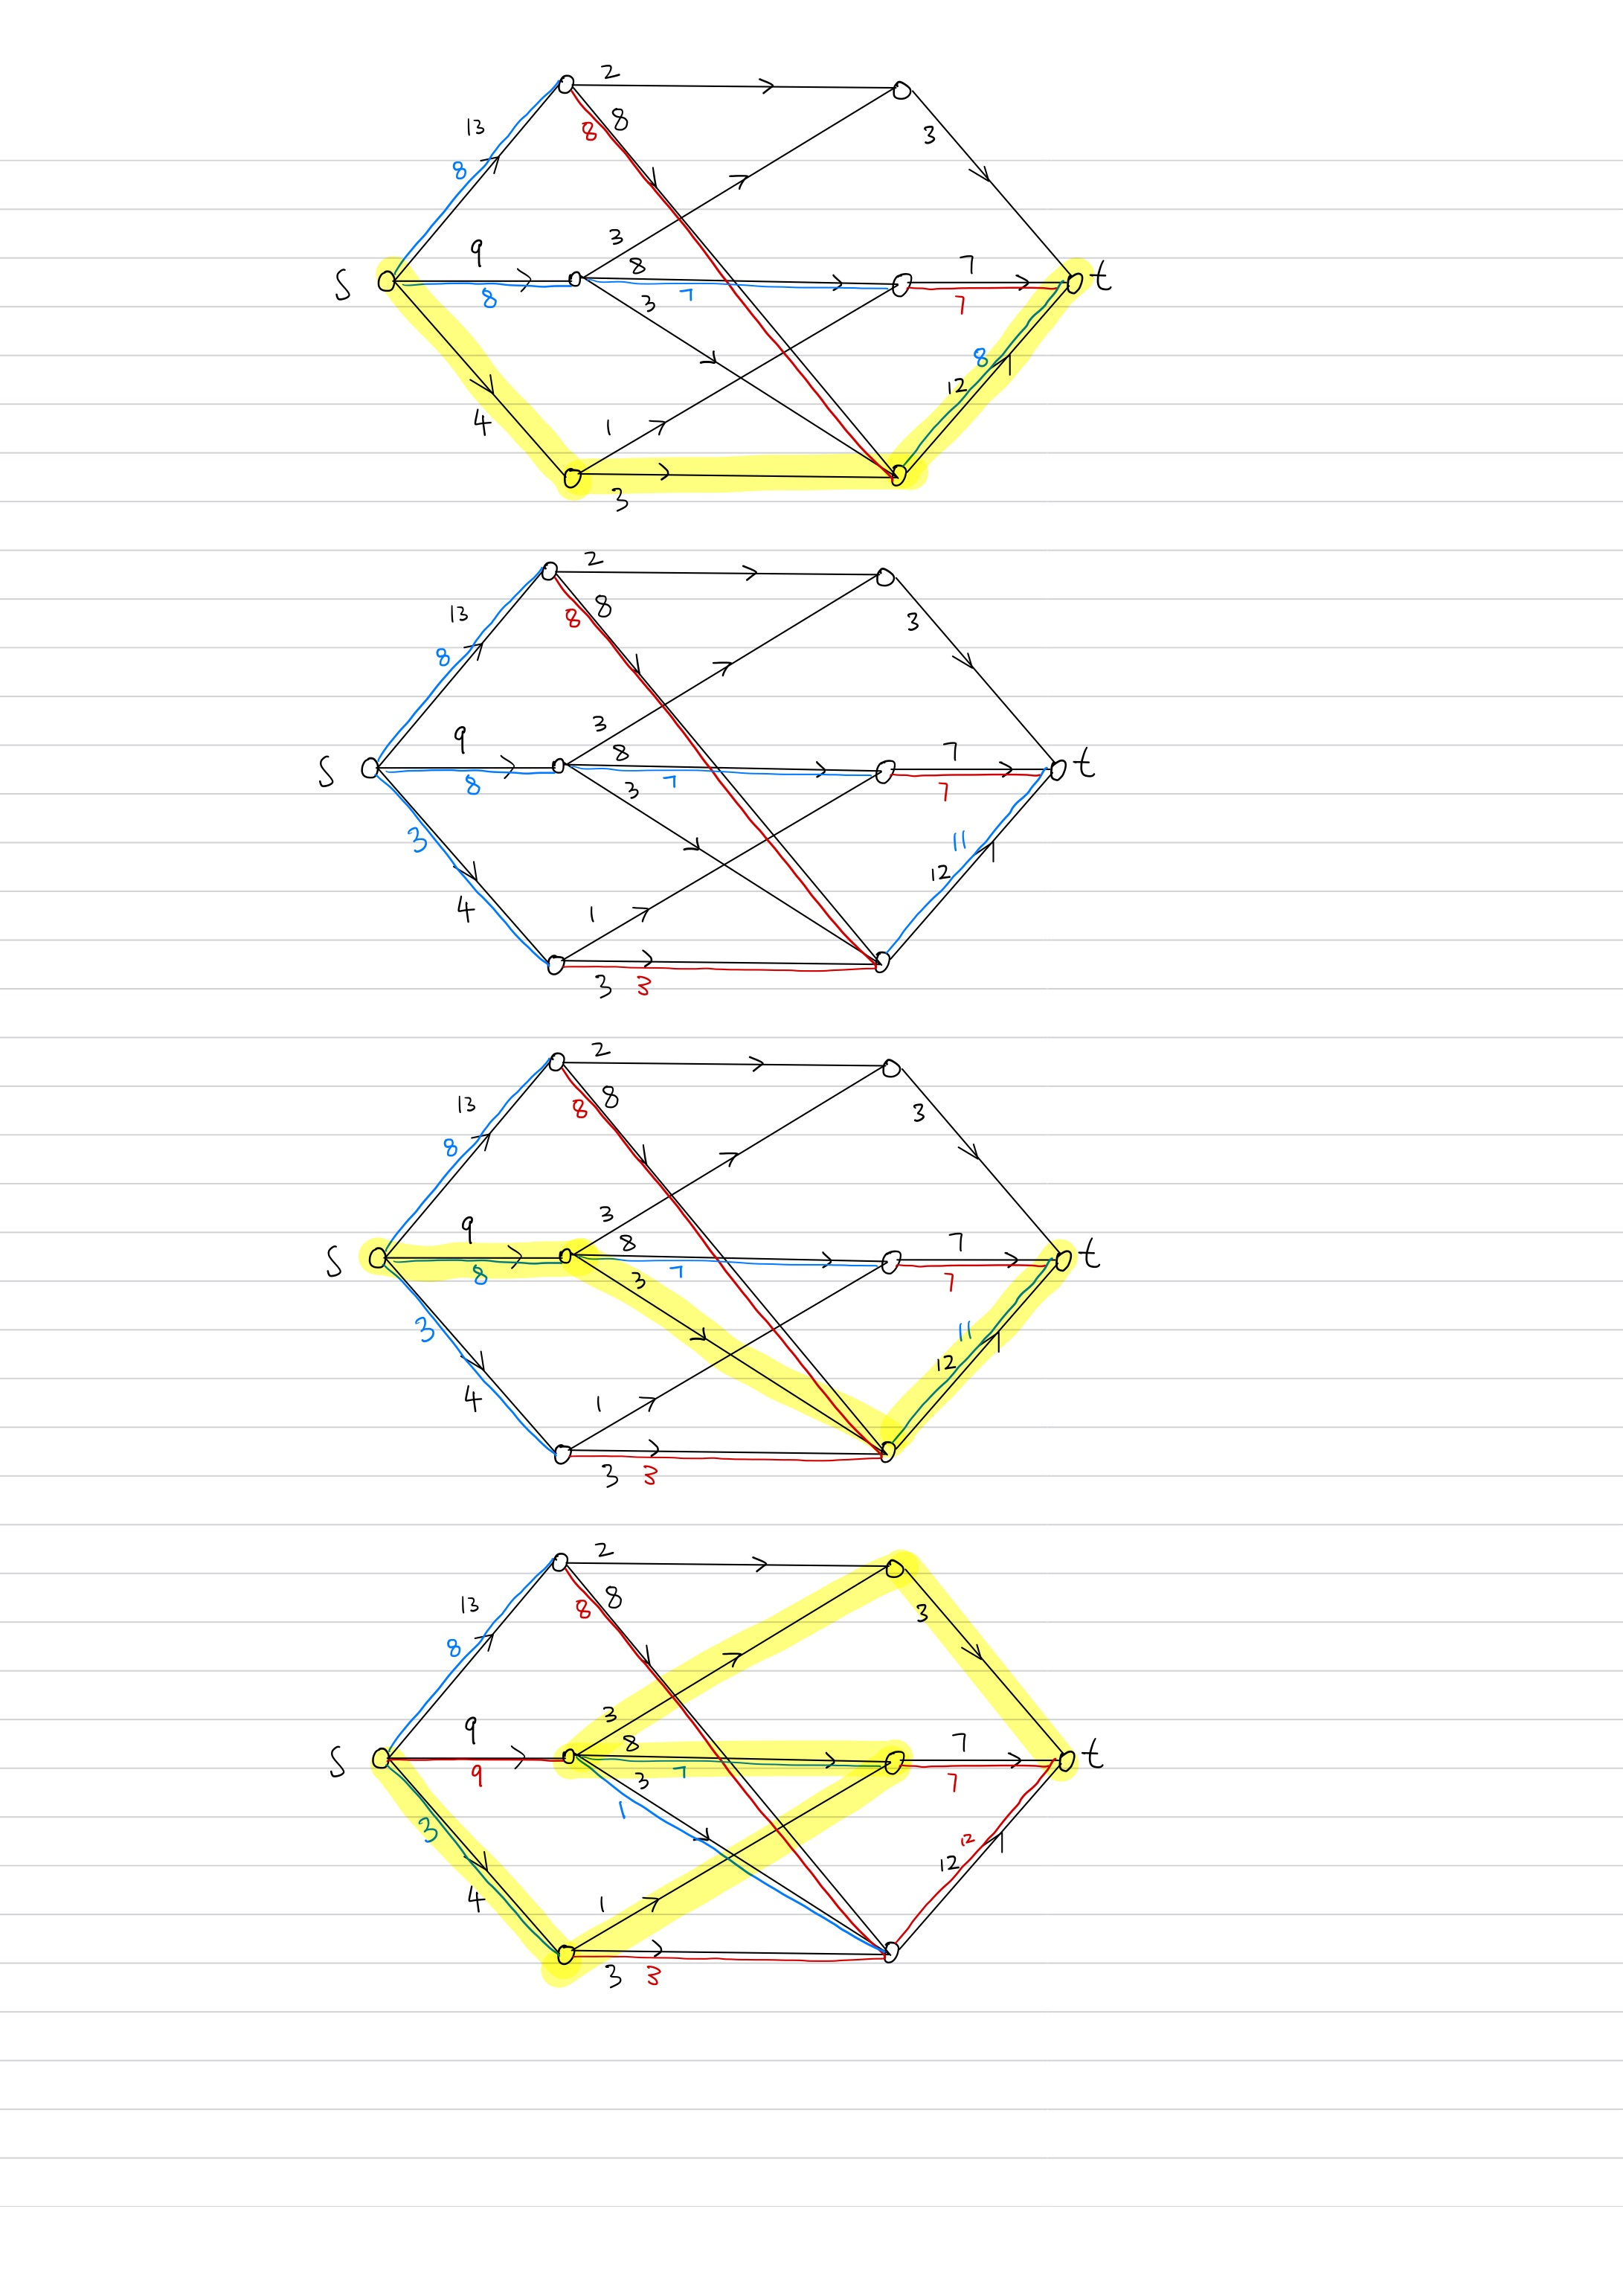
\includegraphics[width=14cm]{Settled Results Ready to Transfer-6.jpg}
        \end{figure}
        \begin{figure}
            \centering
            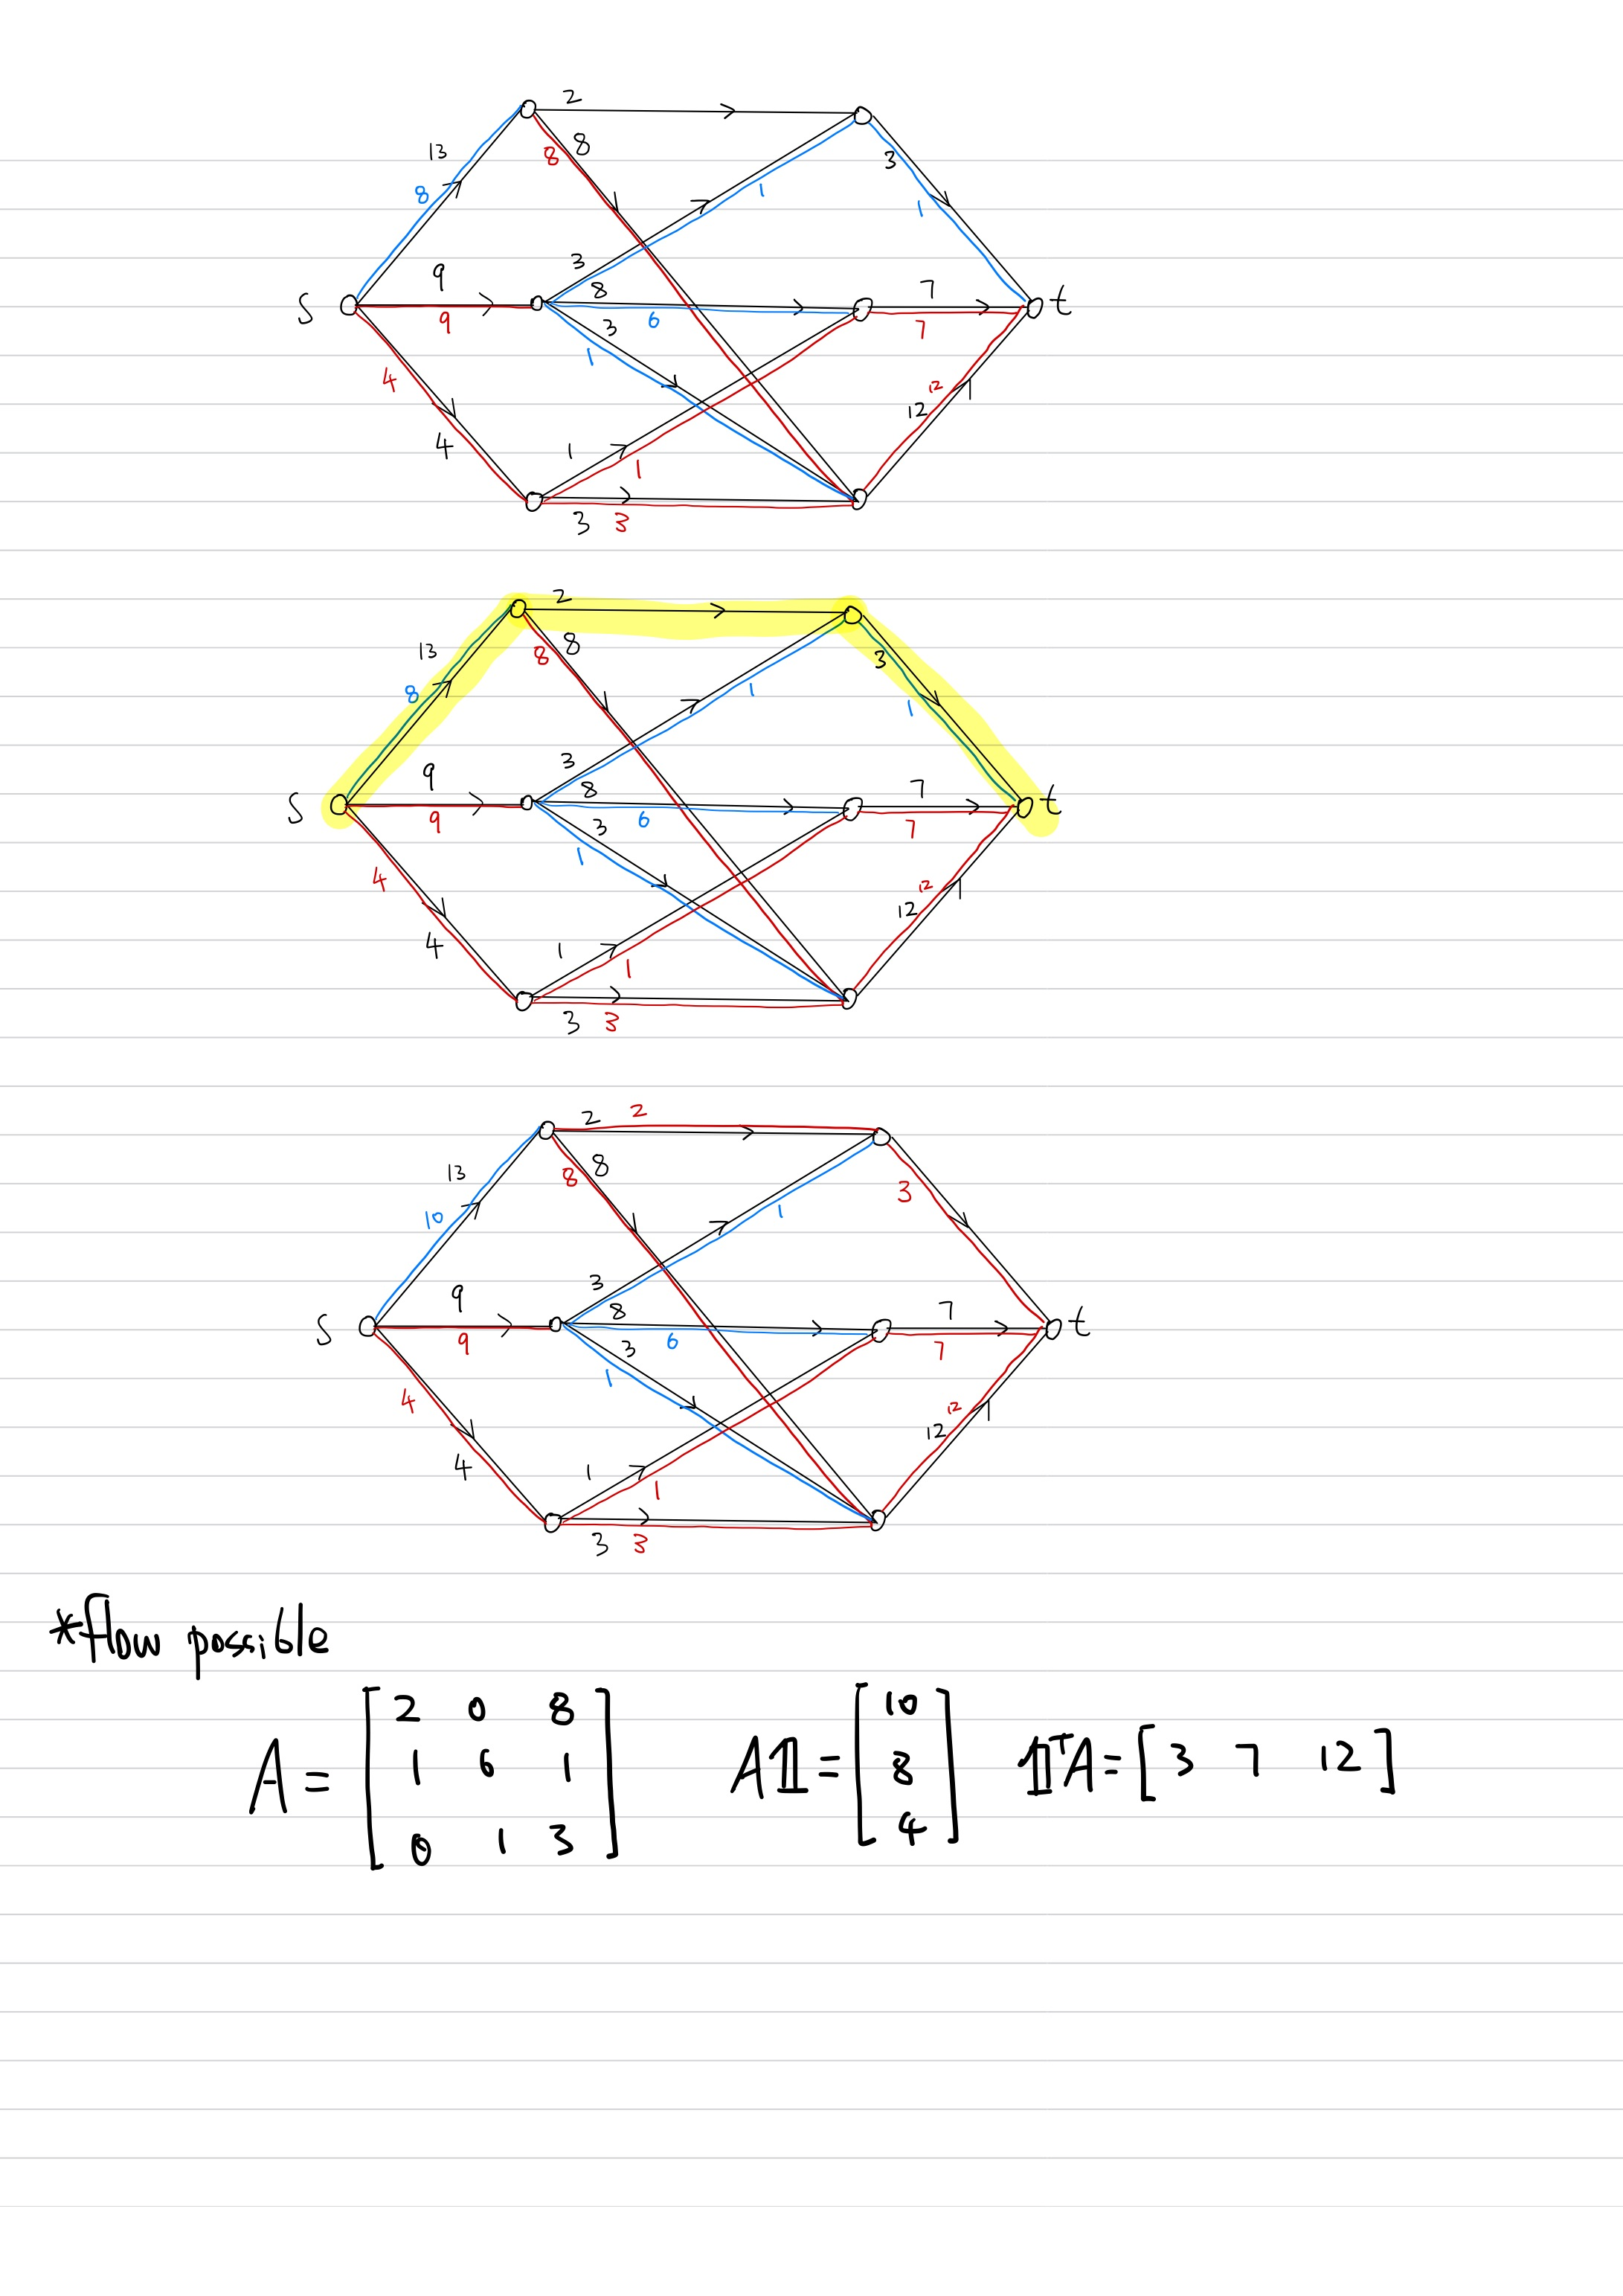
\includegraphics[width=14cm]{Settled Results Ready to Transfer-7.jpg}
        \end{figure}
    \newpage

\section{Problem 4.15}
    \begin{prop}
        Let $D = (V, A)$ be a directed graph, and let $f:A\mapsto \mathbb R_+$, let $\mathcal C$ be the collection of directed circuits in $D$. For each directed circuit $C$ in $D$, let $\chi^C$ be the incidence vector of $C$, that is, $\chi^C: A\mapsto \{0, 1\}$, $(\chi^C)_a=1=\chi^C(a)$ if $C$ traverse the arc $a$ else $\chi^C(a) = 0$. 
        \par
        $f$ is a non-negative circulations if and only if there exists a function $\lambda: \mathcal C \rightarrow \mathbb R_+$ such that: 
        \begin{align}
            f = \sum_{C\in \mathcal C}^{}\lambda(C)\chi^C
        \end{align}
        \par
        Simply put, all non-negative flow on the graph form the cone of all circuits vector on the graph. 
    \end{prop}
    \subsection{Proof of Necessity $\impliedby$}
        We wish to show that the cone of circuits indicators vectors are still a non-negative flow. To characterize non-negative flow on the digraph, we define the incidence matrix $M$ using the following: 
        \begin{align}
            M := \begin{bmatrix}
                \mathbbm 1_{\delta^+(v_1)}^T - \mathbbm 1_{\delta^{-}(v_1)}^T
                \\
                \mathbbm 1_{\delta^+(v_2)}^T - \mathbbm 1_{\delta^{-}(v_2)}^T
                \\
                \vdots 
                \\
                \mathbbm 1_{\delta^+(v_n)}^T - \mathbbm 1_{\delta^{-}(v_n)}^T
            \end{bmatrix}
        \end{align}
        Then the polyhedron $P:=\{x\ge \mathbf 0 | Mx = \mathbf 0\}$ will characterize all the non-negative flow on the graph (This is directly by definition of non-negative flow). Consider any $\chi^C \ge \mathbf 0$, which is non-negative, there sum will be non-negative too. 
        \par
        $C$ is a circuit, therefore $\forall v \in C: \delta^+(v) = \delta^-(v)$, therefore the incidence vector $\chi^C$ has property $M\chi^C = \mathbf 0$. Therefore: 
        \begin{align}
            M \sum_{c \in \mathcal C}^{} \lambda(C)\chi^C = 
            \sum_{c \in \mathcal C}^{} \lambda(C)M\chi^C = \mathbf 0
            \\
            \implies \sum_{c\in C}^{}\lambda(C)\chi^C \in P
        \end{align}
        Therefore, for all element in the cone spanned by the incidence vector of all cirtuits on the graph, it's also in the polyhedron that characterize non-negative flow on the graph. 
    \subsection{Proof of Sufficiency $\implies$}
        Given any non-negative flow, it can be represented by some element in the cone $\text{cone}(\mathcal C)$. If the non-negative circulation is all zero, then it's trivialy true, just make $\lambda(C) = 0 \;\forall\; C$.
        \par
        Next, assuming that the circulation $f^{(0)} = f$ is strictly positive, we use $\chi^{f^{(0)}}$ as an indicator vector to denote all the arc in the circulation, then there must exist $\chi^{C}$ for some $C \in \mathcal C$ such that for all arcs in $C$, it's in $f^{(0)}$. For contradiction if this is not true, then there exist some path where the flow ends at a vertex $v$, making $\sum_{a\in\delta^+(v)} f(a) \neq \sum_{a\in \delta^-(v)}^{}f(a)$, hence $f$ is not a circulation. 
        \par
        Let $C_0$ be the circuit such that for all $a\in C_0: f(a) \ge 0$. Choose $0 <\alpha_1 = \min_{a \in C_0}f(a)$, then: 
        \begin{align}
            f^{(1)} := f^{(0)} - \alpha_1 \chi^{C_0}
        \end{align}
        $f^{(0)}$ is still a circulation. This is true because forall $v\in V$, it's either $v$ is covered by circulation $f^{(0)}$, or it's covered by $f^{(0)}\cup C_0$. In the former case, the flow coming in and out is equal, in the latter case: 
        \begin{align}
            \sum_{a\in\delta^+(v)\cap C_0}^{} f^{(0)}(a) &= \sum_{a\in \delta^-(v)\cap C_0}^{}f^{(0)}(a)
            \\
            \implies \sum_{a\in \delta^+(v)}^{}f^{(0)}(a) - \sum_{a \in \delta^+(v)\cap C_0}^{}\alpha_1 f^{0}(a) &= 
            \sum_{a\in \delta^-(v)}^{}f^{(0)}(a) - \sum_{a \in \delta^-(v)\cap C_0}^{}\alpha_1 f^{(0)}(a) 
        \end{align}
        Therefore $f^{(1)}$ is still a circulation. Let's consider the statement inductively, then one can show that: 
        \begin{align}
            \mathbf 0 < f^{(1)} &:= f^{(0)} - \alpha_1 \chi^{C_0}\quad \alpha_1 := \min_{a \in C_0}f^{(0)}(a)
            \\
            \mathbf 0 < f^{(2)} &:= f^{(1)} - \alpha_2 \chi^{C_0}\quad \alpha_2 := \min_{a \in C_1}f^{(1)}(a)
            \\
            \vdots 
            \\
            \mathbf 0 = f^{(n)} &:= f^{(n - 1)} - \alpha_{n - 1} \chi^{C_{n - 1}} \quad \alpha_{n - 1} := \min_{a \in C_{n - 1}}f^{(n - 1)}(a)
        \end{align}
        The sequence of non-negative circulation will terminates with exactly zero. This is inductively true because all circulation must contain a circuit, if it's not, then it's not a circulation. Therefore, the original initial circulation can be expressed in the form of: 
        \begin{align}
            \mathbf 0 &= f^{(n - 1)} - \alpha_{n - 1} \chi^{C_{n - 1}} 
            \\
            \mathbf 0 &= f^{(n - 2)} - \alpha_{n - 2} \chi^{C_{n - 2}}  - \alpha_{n - 1} \chi^{C_{n - 1}} 
            \\
            \vdots
            \\
            \mathbf 0 &= f^{(0)} - 
            \left(\sum_{j = 1}^{n - 1}\alpha_j\chi^{C_{j}}\right)
        \end{align}
        And we have expresed the non-negative circulation $f^{(0)}$ as a non-negative summation of all the indicator vector for circuits on $D$. All citcuits on $D$ is coming from $\mathcal C$, therefore, all non-negative circulations are inside of $\text{cone}(\mathcal C)$. 

\section{Problem 4.18}
    Describe the problem of finding a max-weighted matching in a bipartite graph as a min-cost flow problem. 
    \subsection{Some Preparations for the Proofs}
        \begin{lemma}[Lemma 1]\label{lemma:1}
            Given a bipartite graph $G:=(V\dot\cup U, E)$, the maximum weight matching of a $w:E \mapsto \mathbb R_+$has to be a maximum cadinality matching first. 
        \end{lemma}
        \begin{proof}
            For contradiction assuming that $M$ is not a maximum cardinality matching and it has maximum weight. Choose $M^+$ that is a maximum cardinality matching, then the set $M^+\Delta M$ is non zero, and there exists edge $e \in M^+$ but $ e\not \in M$. Choosing such an edge and include it to $M$ gives more weight for $M$ because the weights are non-negative. Contradiction is shown. 
        \end{proof}
        We make the notation of converting an arc $a = (u, v)$ into an edge as $E(a) = \{u, v\}$. 
        \par
        The reduction process goes by converting the undirection Bipartite graph into a directed graph, and then convert the weight function into a cost function, and then define the fix amount of flow for the min cost flow algorithm. 
    \subsection{The Reduction Process}
        Given bipartite graph $G:= (U\dot\cup V, E)$, construct: 
        \begin{align}
            A &= \{(u, v)| u\in U\wedge v \in V\}
            \\
            D &:= (\{s, t\}\cup U\dot\cup V, A \cup \{(s, u)| u \in V\}\cup \{(v, t)| v \in V\})   
            \\
            c: E\mapsto \mathbb R_+ &\equiv 1
        \end{align}
        \par
        The amount of flow that we wish to send equals to $|M|$ where $M$ is the maximum cardinality matching on $G$. All edges are having a capacity of 1, therefore there exists maximum value flow solution as an integral flow on the graph $D$.
        \par
        Observe that for all $v \in V$, $\sum_{a \in \delta^+(v)}^{}f(a) \le 1$, and similarly for all $u \in U$, $\sum_{a \in \delta^-(v)}^{}f(u) \le 1$ as well, which implies that all integral maximum flow $f$ on $D$ is a matching, in addition the arcs that is in $f$ and goes between the set $U, V$ will be a maximum cardinality matching between $U, V$. This is true because the value can be computed as: 
        \begin{align}
            \text{val}(f) = \sum_{a\in \delta^+(s)}f(a) = 
            \sum_{v\in V}^{}\sum_{a \in \delta^-{(v)}}f(a) = |M|
        \end{align}
        Next, define the cost function $k(a) = -w(E(a))$, the cost function is just the negative weight. Since w is $\mathbb R_+$, then $k$ is $\mathbb R_-$. Minimizing the cost among all flow with a flow of $|M|$ will correspond to maximumizing the weight for all matching on $G$ with cardinality $|M|$. The solution with maximum weight must has a flow value the same as a matching with max cardinality, this is proved in \hyperref[lemma:1]{lemma \ref*{lemma:1}}, therefore, the minimum cost among all flow must be a flow with a value $|M|$. 

\section{Problem 4}
    
        
        
\end{document}